\section{Application de la SVD à la compression d'image}
Pour terminer, dans cette partie, nous allons appliquer les transformations de matrices vues dans les parties 2 et 3 à 
l'algorithme de compression d'image par factorisation SVD.\\

On cherche à utiliser la compression SVD sur une image contenant 3 composantes : rouge, vert et bleu.
Pour cela, on récupère une matrice d'intensité pour chacune des couleurs, ce qui permet d'appliquer la compression SVD sur chacune des composantes.

Notons $R$, $G$ et $B$ les matrices d'intensités correspondant aux 3 composantes.
Notons $U_r$, $V_r$, $S_r$ les matrices obtenues pour $R$,
$U_g$, $V_g$, $S_g$ les matrices obtenues pour $G$ puis
$U_b$, $V_b$, $S_b$ les matrices obtenues pour $B$.
On a alors $R = U_r \times S_r \times V_r$, $G = U_g \times S_g \times V_g$ et enfin
$B = U_b \times S_b \times V_b$.
\bigbreak
Pour obtenir une compression au rang $r$ sur toutes les composantes, 
on annule tous les termes diagonaux de $S_r$, $S_g$ et $S_b$ d'indices 
strictement supérieurs à $r$, et inférieurs à $min(m, n)$.
En réalité, ce calcul en entraîne un autre : comme on perd de l'information, il se peut que les valeurs dans la nouvelle matrice $U \times S \times V$ deviennent inférieures à 0 ou supérieures à 1 
(ou 255 dans le cas où l'on raisonne sur des entiers).
La solution a donc été de borner les valeurs, et donc de les ramener aux bords du domaine si elles dépassaient du bord.
\bigbreak
En faisant cela, on perd de l'information sur l'image, mais la quantité de données stockées est moins grande.
En effet, pour stocker l'image, au lieu de stocker $n \times m$ données, il suffit de stocker 
les parties de $U$ et $V$ qui n'entraînent pas de produits nuls avec les matrices $S$ (ce qui donne des matrices de taille $k \times m$ et $n \times k$)
en plus des diagonales des matrices $S$ (seule la diagonale suffit puisque ce sont des matrices diagonales).

Notons qu'en enregistrant par exemple $U$ et $S \times V$, on peut éviter d'enregistrer la diagonale de $S$, ce qui donnerait exactement deux matrices de tailles $k \times m$ et $n \times k$.
C'est ce que l'on considère dans la suite.
Dans ce cas, on stocke $3 \times r \times (n + m)$ valeurs.
Cette taille est généralement inférieure à la taille de départ, mais à partir d'une certain rang $r_{lim}$, la compression perd de son sens, pour $r_{lim} = \frac{n \times m}{n + m}$.
\bigbreak

Nous avons tracé la norme de la différence de l'image générée à l'image de départ, en échelle logarithmique en figure~\ref{fig:p4-dist}. De toute évidence, dès que le rang atteint $min(n, m)$,
la différence est nulle.
Nous pouvons remarquer que même avec un rang de compression assez faible, on peut garder un écart très faible à l'image originale.

On peut voir le rang $r_{lim}$ à partir duquel la compression n'est plus intéressante en termes de stockage. Pour ce rang, l'image semble très similaire à celle de base,
mais par exemple pour une compression de rang 110, et le résultat est très similaire, cette méthode est donc intéressante en ce qui concerne le stockage.

\begin{figure}[htbp]
	\centering
	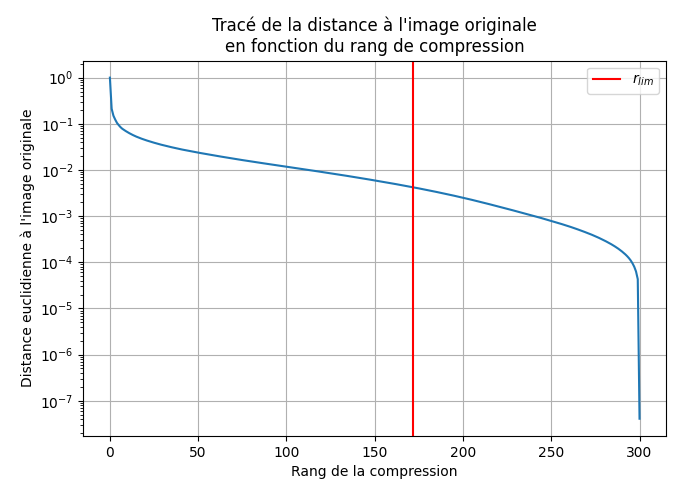
\includegraphics[width=0.65\textwidth]{res/part-4-dist.png}
	\caption{Tracé de l'efficacité de la compression (avec l'image fournie).} 
	\label{fig:p4-dist}
\end{figure}